\documentclass[a4paper]{article}

\def\npart{III}

\def\ntitle{Combinatorics}
\def\nlecturer{I.\ B.\ Leader}

\def\nterm{Michaelmas}
\def\nyear{2018}

\ifx \nauthor\undefined
  \def\nauthor{Qiangru Kuang}
\else
\fi

\ifx \ntitle\undefined
  \def\ntitle{Template}
\else
\fi

\ifx \nauthoremail\undefined
  \def\nauthoremail{qk206@cam.ac.uk}
\else
\fi

\ifx \ndate\undefined
  \def\ndate{\today}
\else
\fi

\title{\ntitle}
\author{\nauthor}
\date{\ndate}

%\usepackage{microtype}
\usepackage{mathtools}
\usepackage{amsthm}
\usepackage{stmaryrd}%symbols used so far: \mapsfrom
\usepackage{empheq}
\usepackage{amssymb}
\let\mathbbalt\mathbb
\let\pitchforkold\pitchfork
\usepackage{unicode-math}
\let\mathbb\mathbbalt%reset to original \mathbb
\let\pitchfork\pitchforkold

\usepackage{imakeidx}
\makeindex[intoc]

%to address the problem that Latin modern doesn't have unicode support for setminus
%https://tex.stackexchange.com/a/55205/26707
\AtBeginDocument{\renewcommand*{\setminus}{\mathbin{\backslash}}}
\AtBeginDocument{\renewcommand*{\models}{\vDash}}%for \vDash is same size as \vdash but orginal \models is larger
\AtBeginDocument{\let\Re\relax}
\AtBeginDocument{\let\Im\relax}
\AtBeginDocument{\DeclareMathOperator{\Re}{Re}}
\AtBeginDocument{\DeclareMathOperator{\Im}{Im}}
\AtBeginDocument{\let\div\relax}
\AtBeginDocument{\DeclareMathOperator{\div}{div}}

\usepackage{tikz}
\usetikzlibrary{automata,positioning}
\usepackage{pgfplots}
%some preset styles
\pgfplotsset{compat=1.15}
\pgfplotsset{centre/.append style={axis x line=middle, axis y line=middle, xlabel={$x$}, ylabel={$y$}, axis equal}}
\usepackage{tikz-cd}
\usepackage{graphicx}
\usepackage{newunicodechar}

\usepackage{fancyhdr}

\fancypagestyle{mypagestyle}{
    \fancyhf{}
    \lhead{\emph{\nouppercase{\leftmark}}}
    \rhead{}
    \cfoot{\thepage}
}
\pagestyle{mypagestyle}

\usepackage{titlesec}
\newcommand{\sectionbreak}{\clearpage} % clear page after each section
\usepackage[perpage]{footmisc}
\usepackage{blindtext}

%\reallywidehat
%https://tex.stackexchange.com/a/101136/26707
\usepackage{scalerel,stackengine}
\stackMath
\newcommand\reallywidehat[1]{%
\savestack{\tmpbox}{\stretchto{%
  \scaleto{%
    \scalerel*[\widthof{\ensuremath{#1}}]{\kern-.6pt\bigwedge\kern-.6pt}%
    {\rule[-\textheight/2]{1ex}{\textheight}}%WIDTH-LIMITED BIG WEDGE
  }{\textheight}% 
}{0.5ex}}%
\stackon[1pt]{#1}{\tmpbox}%
}

%\usepackage{braket}
\usepackage{thmtools}%restate theorem
\usepackage{hyperref}

% https://en.wikibooks.org/wiki/LaTeX/Hyperlinks
\hypersetup{
    %bookmarks=true,
    unicode=true,
    pdftitle={\ntitle},
    pdfauthor={\nauthor},
    pdfsubject={Mathematics},
    pdfcreator={\nauthor},
    pdfproducer={\nauthor},
    pdfkeywords={math maths \ntitle},
    colorlinks=true,
    linkcolor={red!50!black},
    citecolor={blue!50!black},
    urlcolor={blue!80!black}
}

\usepackage{cleveref}



% TODO: mdframed often gives bad breaks that cause empty lines. Would like to switch to tcolorbox.
% The current workaround is to set innerbottommargin=0pt.

%\usepackage[theorems]{tcolorbox}





\usepackage[framemethod=tikz]{mdframed}
\mdfdefinestyle{leftbar}{
  %nobreak=true, %dirty hack
  linewidth=1.5pt,
  linecolor=gray,
  hidealllines=true,
  leftline=true,
  leftmargin=0pt,
  innerleftmargin=5pt,
  innerrightmargin=10pt,
  innertopmargin=-5pt,
  % innerbottommargin=5pt, % original
  innerbottommargin=0pt, % temporary hack 
}
%\newmdtheoremenv[style=leftbar]{theorem}{Theorem}[section]
%\newmdtheoremenv[style=leftbar]{proposition}[theorem]{proposition}
%\newmdtheoremenv[style=leftbar]{lemma}[theorem]{Lemma}
%\newmdtheoremenv[style=leftbar]{corollary}[theorem]{corollary}

\newtheorem{theorem}{Theorem}[section]
\newtheorem{proposition}[theorem]{Proposition}
\newtheorem{lemma}[theorem]{Lemma}
\newtheorem{corollary}[theorem]{Corollary}
\newtheorem{axiom}[theorem]{Axiom}
\newtheorem*{axiom*}{Axiom}

\surroundwithmdframed[style=leftbar]{theorem}
\surroundwithmdframed[style=leftbar]{proposition}
\surroundwithmdframed[style=leftbar]{lemma}
\surroundwithmdframed[style=leftbar]{corollary}
\surroundwithmdframed[style=leftbar]{axiom}
\surroundwithmdframed[style=leftbar]{axiom*}

\theoremstyle{definition}

\newtheorem*{definition}{Definition}
\surroundwithmdframed[style=leftbar]{definition}

\newtheorem*{slogan}{Slogan}
\newtheorem*{eg}{Example}
\newtheorem*{ex}{Exercise}
\newtheorem*{remark}{Remark}
\newtheorem*{notation}{Notation}
\newtheorem*{convention}{Convention}
\newtheorem*{assumption}{Assumption}
\newtheorem*{question}{Question}
\newtheorem*{answer}{Answer}
\newtheorem*{note}{Note}
\newtheorem*{application}{Application}

%operator macros

%basic
\DeclareMathOperator{\lcm}{lcm}

%matrix
\DeclareMathOperator{\tr}{tr}
\DeclareMathOperator{\Tr}{Tr}
\DeclareMathOperator{\adj}{adj}

%algebra
\DeclareMathOperator{\Hom}{Hom}
\DeclareMathOperator{\End}{End}
\DeclareMathOperator{\id}{id}
\DeclareMathOperator{\im}{im}
\DeclareMathOperator{\coker}{coker}
\DeclarePairedDelimiter{\generation}{\langle}{\rangle}

%groups
\DeclareMathOperator{\sym}{Sym}
\DeclareMathOperator{\sgn}{sgn}
\DeclareMathOperator{\inn}{Inn}
\DeclareMathOperator{\aut}{Aut}
\DeclareMathOperator{\GL}{GL}
\DeclareMathOperator{\SL}{SL}
\DeclareMathOperator{\PGL}{PGL}
\DeclareMathOperator{\PSL}{PSL}
\DeclareMathOperator{\SU}{SU}
\DeclareMathOperator{\UU}{U}
\DeclareMathOperator{\SO}{SO}
\DeclareMathOperator{\OO}{O}
\DeclareMathOperator{\PSU}{PSU}
\DeclareMathOperator{\Sp}{Sp}


%hyperbolic
\DeclareMathOperator{\sech}{sech}

%field, galois heory
\DeclareMathOperator{\ch}{ch}
\DeclareMathOperator{\gal}{Gal}
\DeclareMathOperator{\emb}{Emb}



%ceiling and floor
%https://tex.stackexchange.com/a/118217/26707
\DeclarePairedDelimiter\ceil{\lceil}{\rceil}
\DeclarePairedDelimiter\floor{\lfloor}{\rfloor}


\DeclarePairedDelimiter{\innerproduct}{\langle}{\rangle}

%\DeclarePairedDelimiterX{\norm}[1]{\lVert}{\rVert}{#1}
\DeclarePairedDelimiter{\norm}{\lVert}{\rVert}



%Dirac notation
%TODO: rewrite for variable number of arguments
\DeclarePairedDelimiterX{\braket}[2]{\langle}{\rangle}{#1 \delimsize\vert #2}
\DeclarePairedDelimiterX{\braketthree}[3]{\langle}{\rangle}{#1 \delimsize\vert #2 \delimsize\vert #3}

\DeclarePairedDelimiter{\bra}{\langle}{\rvert}
\DeclarePairedDelimiter{\ket}{\lvert}{\rangle}




%macros

%general

%divide, not divide
\newcommand*{\divides}{\mid}
\newcommand*{\ndivides}{\nmid}
%vector, i.e. mathbf
%https://tex.stackexchange.com/a/45746/26707
\newcommand*{\V}[1]{{\ensuremath{\symbf{#1}}}}
%closure
\newcommand*{\cl}[1]{\overline{#1}}
%conjugate
\newcommand*{\conj}[1]{\overline{#1}}
%set complement
\newcommand*{\stcomp}[1]{\overline{#1}}
\newcommand*{\compose}{\circ}
\newcommand*{\nto}{\nrightarrow}
\newcommand*{\p}{\partial}
%embed
\newcommand*{\embed}{\hookrightarrow}
%surjection
\newcommand*{\surj}{\twoheadrightarrow}
%power set
\newcommand*{\powerset}{\mathcal{P}}

%matrix
\newcommand*{\matrixring}{\mathcal{M}}

%groups
\newcommand*{\normal}{\trianglelefteq}
%rings
\newcommand*{\ideal}{\trianglelefteq}

%fields
\renewcommand*{\C}{{\mathbb{C}}}
\newcommand*{\R}{{\mathbb{R}}}
\newcommand*{\Q}{{\mathbb{Q}}}
\newcommand*{\Z}{{\mathbb{Z}}}
\newcommand*{\N}{{\mathbb{N}}}
\newcommand*{\F}{{\mathbb{F}}}
%not really but I think this belongs here
\newcommand*{\A}{{\mathbb{A}}}

%asymptotic
\newcommand*{\bigO}{O}
\newcommand*{\smallo}{o}

%probability
\newcommand*{\prob}{\mathbb{P}}
\newcommand*{\E}{\mathbb{E}}

%vector calculus
\newcommand*{\gradient}{\V \nabla}
\newcommand*{\divergence}{\gradient \cdot}
\newcommand*{\curl}{\gradient \cdot}

%logic
\newcommand*{\yields}{\vdash}
\newcommand*{\nyields}{\nvdash}

%differential geometry
\renewcommand*{\H}{\mathbb{H}}
\newcommand*{\transversal}{\pitchfork}
\renewcommand{\d}{\mathrm{d}} % exterior derivative

%number theory
\newcommand*{\legendre}[2]{\genfrac{(}{)}{}{}{#1}{#2}}%Legendre symbol

%algebraic geometry
\DeclareMathOperator{\Spec}{Spec}
\DeclareMathOperator{\Proj}{Proj}

\let\SO\undefined
\usepackage{tkz-graph}

\newcommand{\shadow}{\partial}
\renewcommand{\P}{\mathbb P}

\begin{document}

\begin{titlepage}
  \begin{center}
    \includegraphics[width=0.6\textwidth]{logo.jpg}\par
    \vspace{1cm}
    {\scshape\huge Mathamatics Tripos \par}
    \vspace{2cm}
    {\huge Part \npart \par}
    \vspace{0.6cm}
    {\Huge \bfseries \ntitle \par}
    \vspace{1.2cm}
    {\Large\nterm, \nyear \par}
    \vspace{2cm}
    
    {\large \emph{Lectures by } \par}
    \vspace{0.2cm}
    {\Large \scshape \nlecturer}
    
    \vspace{0.5cm}
    {\large \emph{Notes by }\par}
    \vspace{0.2cm}
    {\Large \scshape \href{mailto:\nauthoremail}{\nauthor}}
 \end{center}
\end{titlepage}

\tableofcontents

\section{Set systems}

\begin{definition}[set system]\index{set system}
  Let \(X\) be a set. A \emph{set system} on \(X\) (or \emph{family of subsets}) of \(X\) is a family \(\mathcal A \subseteq \powerset (X)\).
\end{definition}

\begin{eg}
  We write \(X^{(r)} = \{A \subseteq X: |A| = r\}\)
\end{eg}

In this course we almost deal exclusively with finite setss so unless otherwise stated, in this course we assume all sets are finite and \(X = [n] = \{1, 2, \dots, n\}\).

For example, \(|X^{(r)}| = \binom{n}{r}\). More concretely, for example,
\[
  [4]^{[2]} = \{12, 13, 14, 23, 24, 34\}
\]
where \(12\) denotes \(\{1, 2\}\) to avoid heavy notation. Therefore \(|[4]^{[2]}| = 6\).

What is the mental picture for power set? Often we make \(\powerset (X)\) into a graph, called \(Q_n\), by joining \(A\) to \(B\) if \(|A \Delta B| = 1\) where \(\Delta\) is the symmetric difference, i.e.\ if \(A = B \cup \{i\}\) for some \(i \notin B\) (or vice verse).

\begin{eg}
  \(Q_3\)
\end{eg}

\begin{eg}
  General picture for \(Q_n\) where \(n\) is even:

  and when \(n\) is odd:
\end{eg}

If we identify a set \(A \subseteq X\) with a \(\{0, 1\}\) sequence of length \(n\) (e.g.\ \(134 \leftrightarrow 1011000 \cdots 0\)), via \(A \leftrightarrow \mathbf{1}_A \text{ or } \chi_A\). In this way, we can represent \(Q_n\) as a \(n\)-dimensional cube:

For this reason, \(Q_n\) is often called the \emph{hypercube} or \emph{discrete cube} or \emph{\(n\)-cube}. In this way, the study of a set system become the study of a graph.

\subsection{Chains \& Antichains}

\begin{definition}[chain]\index{chain}
  A family \(\mathcal A \subseteq \powerset (X)\) is a \emph{chain} if for all \(A, B \in \mathcal A, A \subseteq B \text{ or } B \subseteq A\).
\end{definition}

\begin{eg}
  \(\{12, 125, 123589\}\).
\end{eg}

On the other hand, we have

\begin{definition}[antichain]\index{antichain}
  A family \(\mathcal A \subseteq \powerset (X)\) is an \emph{antichain} if for all \(A, B \in \mathcal A\) with \(A \neq B\), \(A \nsubseteq B\).
\end{definition}

\begin{eg}
  \(\{1, 467, 2456\}\).
\end{eg}

A natural question is: how large can a chain be? Obviously we can achieve \(|\mathcal A| = n + 1\). We also cannot exceed \(n + 1\) since a chain must meet each ``level'' \(X^{(r)}\) for \(0 \leq r \leq n\) in at most one place.

A less trivial question is how large an antichain can be. We could achieve \(|\mathcal A| = n\) by enumerating all the singletons. It is maximal since adjoining any nonempty set to the family will result in an inclusion. However, it is not the largest antichain. Indeed, we could take \(\mathcal A = X^{(r)}\) for any \(r\). Thus we can achieve \(|\mathcal A| = \binom{n}{\floor{n/2}}\). Can we beat it?

Pause for a moment and consider the longest chain problem. Why can a chain meet each level at only one place? One way to see this is that each level is an antichain: as we can decompose \(Q_n\) into \(n + 1\) antichains, we cannot have a chain longer than that. Inspired by this, we try to decompose \(Q_n\) into chains.

\begin{theorem}[Sperner's lemma]\index{Sperner's lemma}
  Let \(\mathcal A \subseteq \powerset(X)\) where \(|X| = n\) be an antichain. Then
  \[
    |\mathcal A| \leq \binom{n}{\floor{n/2}}.
  \]
\end{theorem}

\begin{proof}
  Sufficient to partition \(\powerset(X)\) into \(\binom{n}{\floor{n/2}}\) chains. For this sufficient to show:
  \begin{enumerate}
  \item for all \(r < \frac{n}{2}\), there exist matchings from \(X^{(r)}\) to \(X^{(r + 1)}\) where a matching is just a set of non-adjacent edges,
  \item for all \(r > \frac{n}{2}\), there exist matchings from \(X^{(r)}\) to \(X^{(r - 1)}\).
  \end{enumerate}
  Then put these matchings together to form chains. Each passes through \(X^{(n/2)}\) so there are \(\binom{n}{\floor{n/2}}\) of them.

  By taking complements, sufficient to prove 1. Consider the subgraph of \(Q_n\) spanned by \(X^{(r)} \cup X^{(r + 1)}\) which is bipartite. For any \(\mathcal B \subseteq X^{(r)}\), let \(\Gamma(\mathcal B)\) be the neighbourhood (in \(X^{(r + 1)}\)) of \(\mathcal B\). Then we have

  \[
    \# (\mathcal B - \Gamma(\mathcal B) \text{ edges}) = |\mathcal B| (n - r)
  \]
  as each point in \(X^{(r)}\) has degree \(n - r\). Meanwhile
  \[
    \# (\mathcal B - \Gamma(\mathcal B) \text{ edges}) \leq |\Gamma(\mathcal B)| (r + 1)
  \]
  as each point in \(X^{(r + 1)}\) has degree \(r + 1\). Thus
  \[
    |\Gamma(\mathcal B)| \geq |\mathcal B| \frac{n - r}{r + 1} \geq |\mathcal B|
  \]
  as \(r < \frac{n}{2}\). Hence by Hall's theorem there exist matchings.
\end{proof}

\begin{remark}\leavevmode
  \begin{enumerate}
  \item \(\binom{n}{\floor{n/2}}\) is achieveable, e.g.\ \(\mathcal A = X^{(\floor{n/2})}\).
  \item Note that the theorem says nothing about extremal cases --- which antinchain have this size?
  \end{enumerate}
\end{remark}

The aim is to show that for \(\mathcal A\) an antichain,
\[
  \sum_{r = 0}^n \frac{\mathcal A \cap X^{(r)}}{\binom{n}{r}} \leq 1.
\]
Note that this trivially implies Sperner's lemma. We will use the same setup but bound the numbers more carefully. To justify the following definition, we will write \(X^{(r)}\) above \(X^{(r - 1)}\) in \(Q_n\).

\begin{definition}
  Let \(\mathcal A \subseteq X^{(r)}\) for some \(1 \leq r \leq n\). The \emph{shadow} or \emph{lower shadow} of \(\mathcal A\) is
  \[
    \shadow A = \shadow^- A = \{A - \{i\}: A \in \mathcal A, i \in A\}.
  \]
  so \(\shadow A \subseteq X^{(r - 1)}\).
\end{definition}

\begin{eg}
  Let \(\mathcal A = \{123, 124, 134, 135\} \subseteq X^{(3)}\). Then
  \[
    \shadow A = \{12, 13, 23, 14, 24, 34, 15, 35\} \subseteq X^{(2)}.
  \]
\end{eg}

\begin{lemma}[Local LYM]\index{local LYM}
  Let \(\mathcal A \subseteq X^{(r)}\) where \(1 \leq r \leq n\). Then
  \[
    \frac{|\shadow \mathcal A|}{\binom{n}{r - 1}} \geq \frac{|\mathcal A|}{\binom{n}{r}}.
  \]
\end{lemma}

Informally, the fraction of the later occupied increases when we take the shadow.

\begin{proof}
  \[
    \#(\mathcal A - \shadow \mathcal A \text{ edges in } Q_n) = r|\mathcal A|
  \]
  by counting from above and
  \[
    \#(\mathcal A - \shadow \mathcal A \text{ edges in } Q_n) \leq (n - r + 1) |\shadow \mathcal A|
  \]
  counting from below so
  \[
    \frac{|\shadow \mathcal A|}{|\mathcal A|} \geq \frac{r}{n - r + 1}
  \]
  but
  \[
    \frac{\binom{r}{r - 1}}{\binom{n}{r}} = \frac{r}{n - r + 1}.
  \]
\end{proof}

When does equality hold in local LYM? We'll need
\[
  (A - \{i\}) \cup \{j\} \in \mathcal A
\]
for all \(a \in \mathcal A, i \in A, j \notin A\). Hence \(\mathcal A = X^{(r)}\) or \(\emptyset\).

\begin{theorem}[LYM inequality]\index{LYM inequality}
  Let \(\mathcal A \subseteq \powerset(X)\) be an antichain. Then
  \[
    \sum_{r = 0}^n \frac{\mathcal A \cap X^{(r)}}{\binom{n}{r}} \leq 1.
  \]
\end{theorem}

\begin{proof}
  The whole idea of the proof can be summarised by ``bubble down with local LYM''. Let \(\mathcal A_r = \mathcal A \cap X^{(r)}\). Obviously
  \[
    \frac{|\mathcal A_n|}{\binom{n}{n}} \leq 1.
  \]
  Also \(\shadow \mathcal A_n\) and \(\mathcal A_{n - 1}\) are distinct as \(\mathcal A\) is an antichain. Thus
  \[
    \frac{|\shadow \mathcal A_n|}{\binom{n}{n - 1}} + \frac{|\mathcal A_{n - 1}|}{\binom{n}{n - 1}}
    = \frac{|\shadow \mathcal A_n \cup \mathcal A_{n - 1}|}{\binom{n}{n - 1}} \leq 1
  \]
  so
  \[
    \frac{|\mathcal A_n|}{\binom{n}{n}} + \frac{|\mathcal A_{n - 1}|}{\binom{n}{n - 1}} \leq 1
  \]
  by local LYM.

  Also \(\shadow (\shadow \mathcal A_n \cup \mathcal A_{n - 1})\) is distint from \(\mathcal A_{n - 2}\), again since \(\mathcal A\) is an antichain. Thus
  \[
    \frac{|\shadow (\shadow \mathcal A_n \cup \mathcal A_{n -1})|}{\binom{n}{n - 2}} +\frac{|\mathcal A_{n - 2}|}{\binom{n}{n - 2}} \leq 1,
  \]
  so
  \[
    \frac{|\shadow \mathcal A_n \cup \mathcal A_{n - 1}|}{\binom{n}{n - 1}} + \frac{|\mathcal A_{n - 1}|}{\binom{n}{n - 2}} \leq 1,
  \]
  so
  \[
    \frac{|\mathcal A_n|}{\binom{n}{n}} + \frac{|\mathcal A_{n - 1}|}{\binom{n}{n - 1}} + \frac{|\mathcal A_{n - 2}|}{\binom{n}{n - 2}} \leq 1
  \]
  Keep going we have the result desired.
\end{proof}

Again we can ask when we have equality in LYM inequality. This happens if and only if we have equality in each use of local LYM, so the ``first'' (greatest) \(r\) with \(\mathcal A_r \neq \emptyset\) must have \(\mathcal A_r = X^{(r)}\) so \(\mathcal A = X^{(r)}\). Thus we know equality in Sperner's lemma (\(\mathcal A = X^{(n/2)}\) for \(n\) even, similar for \(n\) odd)

\begin{proof}[Proof 2]
  Choose uniformly at random a maximal chain \(\mathcal C\) (i.e.\ \(C_0 \subseteq C_1 \subseteq \dots \subseteq C_n\) with \(|C_i| = i\)). For a given \(r\)-set \(A\), \(\P(A \in \mathcal C) = \binom{n}{r}^{-1}\) as all \(r\)-sets are equally likely. Therefore
  \[
    \P(\mathcal A_r \text{ meets } \mathcal C) = \frac{|\mathcal A_r|}{\binom{n}{r}}
  \]
  since the events are disjoint. Furthermore for different \(r\) the events that \(\mathcal A\) meets \(X^r\) are also disjoint so
  \[
    \P(\mathcal A \text{ meets } \mathcal C) = \sum_{r = 0}^n \frac{|\mathcal A_r|}{\binom{n}{r}}
  \]
  and of course it is less than \(1\).
\end{proof}

%how do we think of the first line (from which the rest follows)? inspired by the first proof of LYM %maybe no?

\begin{remark}
  Equivalently, the number of maximal chains is \(n!\) and the number of them containing a given \(r\)-set is \(r! (n - r)!\), so
  \[
    \sum_{r = 0}^n |\mathcal A_r| r! (n - r)! \leq n!
  \]
  so this is probability in disguise
\end{remark}

\subsection{Shadows}

For \(\mathcal A \subseteq X^{(r)}\), we know \(|\shadow A| \geq |A| \frac{r}{n - r + 1}\) --- but equality is rare (only for \(\mathcal A = \emptyset\) or \(\mathcal A = X^{(r)}\)). The natural question is: given \(|\mathcal A|\), how should we choose \(\mathcal A \subseteq X^{(r)}\) to minimise \(|\shadow A|\)? Informally, this asks how ``tightly'' can we pack some \(r\)-sets.

If \(|A| = \binom{k}{r}\), it is believable that we would take \(A = [k]^{(r)}\), which gives \([k]^{(r - 1)}\). What if \(\binom{k}{r} < |\mathcal A| <\binom{k + 1}{r}\), it is believable that we'd take \([k]^{(r)}\) and some other \(r\)-sets from \([k + 1]^{(r)}\). For example if \(\mathcal A \subseteq X^{(3)}\) with \(|\mathcal A| = \binom{7}{3} + \binom{4}{2}\), we would take
\[
  \mathcal A = [7]^{(3)} \cup \{A \cup \{8\}: A \in [4]^{(2)}\},
\]
i.e.\ take those in \([7]\) of size \(3\) so that they are as tightly packed as possible and then choose some other stuff.

If we increment the size of \(\mathcal A\) by \(1\), it is believable that we should take the above \(\mathcal A\) and adjoin another element from \([4]\). Thus it seems that there is a total order on subsets of \(X\) of a given size, and we just take the first \(|\mathcal A|\).

\subsubsection{Two total orderings on \(X^{(r)}\)}

\begin{definition}[lexicographic order]\index{lexicographic order}
  Given \(A, B \in X^{(r)}\), say \(A = a_1, \dots, a_r, B = b_1, \dots, b_r\), where we use the notation to mean \(a_1 < \dots < a_r\), say \(A < B\) in the \emph{lexicographic} or \emph{lex} order if for some \(i\) have \(a_i < b_i\) and \(a_j = b_j\) for all \(j < i\).
\end{definition}

Equivalently, \(a_i < b_i\), where \(i = \min\{j: a_j \neq b_i\}\). The slogan is ``use small number''.

\begin{eg}
  Lex on \([4]^{(2)}\):
  \[
    12, 13, 14, 23, 24, 34.
  \]

  Lex on \([6]^{(3)}\):
  \begin{align*}
    &123, 124, 125, 126, 134, 135, 136, 145, 146, 156, \\
    &234, 235, 236, 245, 246, 256, 345, 346, 356, 456.
  \end{align*}
\end{eg}

However, in the shadow minimisation problem we want to avoid large numbers as much as possible, i.e.\ keep the largest number as small as possible.

\begin{definition}[colexicographic order]\index{colexicographic order}
  Say \(A < B\) isn the \emph{colexicographic} or \emph{colex} order if for some \(i\) have \(a_i < b_i\) and \(a_j = b_j\) for all \(j > i\).
\end{definition}

Equivalently, \(a_i < b_i\) where \(i = \max\{j: a_j \neq b_j\}\). The slogan is ``avoid large number''. Equivalently, \(A < B\) if \(\sum_{i \in A} 2^i < \sum_{i \in B} 2^i\).

\begin{eg}
  Colex on \([4]^{(2)}\):
  \[
    12, 13, 23, 14, 24, 34.
  \]

  Colex on \([6]^{(2)}\):
  \begin{align*}
    &123, 124, 134, 234, 125, 135, 235, 145, 245, 345,\\
    &126, 136, 236, 146, 246, 346, 156, 256, 356, 456.
  \end{align*}
\end{eg}

\begin{note}
  In colex, \([k]^{(r)}\) is an initial segment of \([k + 1]^{(r)}\), meaning that it is the first \(t\) elements for some \(t\). Therefore we could view colex as an enumeration of \(\N^{(r)}\). Try this with lex and see what happens!
\end{note}

Following our heuristics just now, the aim is to show initial segments of cloex minimise \(\shadow\), i.e.\ if \(\mathcal A \subseteq X^{(r)}\) and \(\mathcal C \subseteq X^{(r)}\) is the first \(|\mathcal A|\) \(r\)-sets in colex then \(|\shadow \mathcal A| \geq |\shadow \mathcal C|\), This is Kruskal-Katona theorem, the first theorem in combinatorics.
In particular, \(|\mathcal A| = \binom{k}{r}\) implies \(|\shadow \mathcal A| \geq \binom{k}{r - 1}\). However, unless \(\mathcal A\) is written in very nice form, it is very difficult to estimate \(\shadow \mathcal A\).

\subsubsection{Compressions}

The idea is to ``replace'' \(\mathcal A \subseteq X^{(r)}\) with some \(\mathcal A' \subseteq X^{(r)}\) such that
\begin{enumerate}
\item \(|\mathcal A'| = |\mathcal A|\),
\item \(|\shadow \mathcal A'| \leq |\shadow \mathcal A|\),
\item \(\mathcal A'\) ``looks more like \(\mathcal C\)'' than \(\mathcal A\) did.
\end{enumerate}

Ideally, we would compress
\[
  \mathcal A \to \mathcal A' \to \mathcal A'' \to \dots \to \mathcal B
\]
where either \(\mathcal B = \mathcal C\), or \(\mathcal B\) is so similar to \(\mathcal C\) that we can see directly that \(|\shadow \mathcal B| \geq |\shadow \mathcal C|\).

\paragraph{Colex prefers \(1\) to \(2\)}

\begin{definition}[\(ij\)-compression]\index{\(ij\)-compression}
  For \(1 \leq i < j \leq n\), the \emph{\(ij\)-compression} \(C_{ij}\) is defined by for \(A \subseteq X\),
  \[
    C_{ij} (A) =
    \begin{cases}
      A - j + i & \text{if } j \in A, i \notin A \\
      A & \text{otherwise}
    \end{cases}
  \]
  and for \(\mathcal A \subseteq \powerset(X)\),
  \[
    C_{ij} (\mathcal A) = \{C_{ij}(A): A \in \mathcal A\} \cup \{A \in \mathcal A: C_{ij}(A) \in \mathcal A\}.
  \]
\end{definition}

\begin{eg}
  If \(\mathcal A = \{123, 134, 234, 235, 247\}\), then
  \[
    C_{12}(\mathcal A) = \{123, 134, 234, 135, 147\}.
  \]
\end{eg}

\(|C_{ij}(\mathcal A)| = |\mathcal A|\) and after the compression it looks ``more'' like colex than lex. Say \(\mathcal A\) is \emph{\(ij\)-compressed} if \(C_{ij}(\mathcal A) = \mathcal A\). It is also intuitively obvious that the operation is indeed a compression in the sense that it decreases the shadow.

\begin{proposition}
  \label{prop:ij-compression}
  Let \(\mathcal A \subseteq X^{(r)}\), \(1 \leq i < j \leq n\) then
  \[
    |\shadow C_{ij}(\mathcal A)| \leq |\shadow \mathcal A|.
  \]
\end{proposition}

\begin{proof}
  Write \(\mathcal A'\) for \(C_{ij} (\mathcal A)\). We'll show that if \(B \in \shadow \mathcal A' - \shadow \mathcal A\) then \(i \in B, j \neq B\) and \(B \cup j - i \in \shadow \mathcal A - \shadow \mathcal A'\) (so \(B\) has a preimage under \(C_{ij}\)). Then done.

  We have \(B \cup x \in \mathcal A'\) for some \(x \notin B\) and \(B \cup x \notin \mathcal A\). Hence \(i \in B \cup x, j \notin B \cup x\) and \((B \cup x) \cup j - i \in \mathcal A\) (so \(B \cup x\) is the set that has been compressed). Note that \(x \neq i\) else \(B \cup j \in \mathcal A\), contradicting \(B \notin \shadow \mathcal A\).

  Certainly \(B \cup j - i \in \shadow \mathcal A\). Claim that \(B \cup j - i \notin \shadow \mathcal A'\), thereby completing the proof: suppose \((B \cup j - i) \cup y \in \mathcal A'\). We cannot have \(y = i\), else \(B \cup j \in \mathcal A'\), whence \(B \cup j \in \mathcal A\), contradiction. Thus \(j \in (B \cup j - i) \cup y\) and \(i \notin (B \cup j - i) \cup y\), so \((B \cup j - i) \cup y \in \mathcal A\) and \(B \cup y \in \mathcal A\) by definition of \(C_{ij}\). Contradiction.
\end{proof}

\begin{remark}
  We have actually showed that
  \[
    \shadow C_{ij}(\mathcal A) \subseteq C_{ij} (\shadow \mathcal A),
  \]
  ``shadow of compression lives inside compression of shadow''.
\end{remark}

\begin{definition}[left-compressed]\index{left-compressed}
  Say \(\mathcal A \subseteq X^{(r)}\) is \emph{left-compressed} if \(C_{ij}(\mathcal A) = \mathcal A\) for all \(i < j\).
\end{definition}

\begin{proposition}
  \label{prop:left compression decreases shadow}
  Let \(\mathcal A \subseteq X^{(r)}\). Then there exists left-compressed \(\mathcal B \subseteq X^{(r)}\) with \(|\mathcal B| = |\mathcal A|\) and \(|\shadow \mathcal B| \leq |\shadow \mathcal A|\).
\end{proposition}

\begin{proof}
  Morally we only have to show that any sequence of compression terminate. Among all \(\mathcal B \subseteq X^{(r)}\) with \(|\mathcal B| = |\mathcal A|\) and \(|\shadow \mathcal B| \leq |\shadow \mathcal A|\), choose one with
  \[
    \sum_{A \in \mathcal B} \sum_{x \in A} x
  \]
  minimal. Then \(\mathcal B\) is left compressed, as if \(C_{ij}(\mathcal B) \neq \mathcal B\) then we contradict minimality.
\end{proof}

\begin{note}\leavevmode
  \begin{enumerate}
  \item Alternatively, we may apply one \(C_{ij}\) then another and so on --- it must terminate.
  \item In fact we can apply each \(C_{ij}\) at most once if we choose a sensible order.
  \end{enumerate}
\end{note}

Certainly initial segments of colex are left-compressed. The converse is blatantly false, e.g.\ \(A = \{123, 124, 125, 126, 127\}\). We need to do more.

\paragraph{colex prefers \(23\) to \(14\)}

We can compress not only singletons but also sets of larger sizes:

\begin{definition}[\(UV\)-compression]\index{\(UV\)-compression}
  For \(U, V \subseteq X\) with \(|U| = |V|\) and \(U \cap V = \emptyset\), the \emph{\(UV\)-compression} \(C_{UV}\) is defined by for \(A \subseteq X\),
  \[
    C_{UV} (A) =
    \begin{cases}
      A \cup U - V & \text{if } V \subseteq A, U \cap A = \emptyset \\
      A & \text{otherwise}
    \end{cases}
  \]
  and for \(\mathcal A \subseteq X^{(r)}\),
  \[
    C_{UV} (\mathcal A) = \{C_{UV}(A): A \in \mathcal A\} \cup \{A \in \mathcal A: C_{UV}(A) \in \mathcal A\}.
  \]
\end{definition}

\begin{eg}
  If \(\mathcal A = \{123, 134, 235, 145, 146, 157\}\), then
  \[
    C_{23, 14}(\mathcal A) = \{123, 134, 235, 145, 236, 157\}.
  \]
\end{eg}

Similar observation: \(|C_{UV}(\mathcal A)| = |\mathcal A|\). Say \(\mathcal A\) is \emph{\(UV\)-compressed if \(C_{UV}(\mathcal A) =\mathcal A\)}. Sadly, \(C_{UV}\) need \emph{not} decrease shadow --- e.g.\ \(\mathcal A = \{146, 467\}\) then \(C_{23, 14}(\mathcal A) = \{236, 467\}\) so \(|\shadow \mathcal A| = 5, |\shadow C_{23, 14}(\mathcal A)| = 6\). Intuitively, removing one elements and adding another sends a set to a ``close neighbour'' which shares largely the same shadow, but once we start doing \(UV\)-compression, some things are ``moved a long way''.

However, note that \(\mathcal A\) in the above example is not left-compressed. It turns out once you have done the ``smaller'' compressions, doing a larger compression always decrease the shadow. Formally,

\begin{proposition}
  \label{prop:UV-compression}
  Let \(\mathcal A \subseteq X^{(r)}\) and \(U,V \subseteq X\) with \(|U| = |V|\) and \(U \cap V = \emptyset\). Suppose that for all \(x \in U\) exists \(y \in V\) such that \(\mathcal A\) is \((U - x, V - y)\)-compressed then
  \[
    |\shadow C_{UV}(\mathcal A)| \leq |\shadow \mathcal A|.
  \]
\end{proposition}

\begin{proof}
  Write \(\mathcal A'\) for \(C_{UV}(\mathcal A)\). Given \(B \in \shadow \mathcal A' - \shadow \mathcal A\), we'll show that \(U \subseteq B, V \cap B = \emptyset\) and \(B \cup V - U \in \shadow \mathcal A - \shadow \mathcal A'\).

  We have \(B \cup x \in \mathcal A'\) for some \(x \notin B\), with \(B \cup x \notin \mathcal A\). So \(U \subseteq B \cup x, V \cap (B \cup x) = \emptyset\) and \((B \cup x) \cup V - U \in \mathcal A\). Thus certainly \(V \cap B = \emptyset\).

  If \(x \in U\), have \(\mathcal A\) is \((U - x, V - y)\)-compressed for some \(y \in V\) so from \((B \cup x) \cup V - U \in \mathcal A\) we obtain \(B \cup y \in \mathcal A\), contradicting \(B \notin \shadow \mathcal A\). Hence \(x \notin U\) and so \(U \subseteq B\). Also \(B \cup V - U \in \shadow \mathcal A\) (as \((B \cup x) \cup V - U \in \mathcal A\)).

  Suppose \(B \cup V - U \in \shadow \mathcal A'\) then \((B \cup V - U) \cup w \in \mathcal A'\) for some \(w\).
  \begin{enumerate}
  \item if \(w \notin U\), then \(V \subseteq (B \cup V - U) \cup w\) and \(U \cap ((B \cup V - U) \cup w) = \emptyset\) so from \((B \cup V - U) \cup w \in \mathcal A'\) we conclude that both \((B \cup V - U) \cup w \in \mathcal A\) and \(B \cup w \in \mathcal A\), contradicting \(B \notin \shadow \mathcal A\).
  \item if \(w \in U\), we have \(\mathcal A\) is \((U - w, V - z)\)-compressed for some \(z \in V\). From \((B \cup V - U) \cup w \in \mathcal A\) (as it is in \(\mathcal A'\) and contains \(V\), so could not have moved), we deduce \(B \cup z \in \mathcal A\), contradicting \(B \notin \shadow \mathcal A\).
  \end{enumerate}
\end{proof}

\begin{remark}
  We have actually showed that
  \[
    \shadow C_{UV}(\mathcal A) \subseteq C_{UV}(\shadow \mathcal A).
  \]
\end{remark}

\begin{theorem}[Krustal-Katona]\index{Krustal-Katona theorem}
  \label{thm:Krustal-Katona}
  Let \(\mathcal A \subseteq X^{(r)}\) where \(1 \leq r \leq n\) and let \(\mathcal C\) be the initial segment of colex on \(X^{(r)}\) with \(|\mathcal C| = |\mathcal A|\), then
  \[
    |\shadow \mathcal A| \geq |\shadow \mathcal C|.
  \]
  In particular if \(|\mathcal A| = \binom{k}{r}\) then
  \[
    |\shadow \mathcal A| \geq \binom{k}{r - 1}.
  \]
\end{theorem}

\begin{proof}
  Let
  \[
    \Gamma = \{(U, V): U, V \subseteq X, |U| = |V| > 0, U \cap V = \emptyset, \max U < \max V\}
  \]
  which are the ordered pairs \((U, V)\) with \(U < V\) in colex, which are exactly the sensible pairs to do \(UV\) compression on in order to decrease shadow. Define a sequence of set systems \(\mathcal A_0, \mathcal A_1, \dots\) in \(X^{(r)}\) as follow:
  \begin{enumerate}
  \item \(\mathcal A_0 = \mathcal A\).
  \item If \(\mathcal A_k\) is \((U, V)\)-compressed for all \((U, V) \in \Gamma\), then stop the sequence with \(\mathcal A_k\).
  \item If not, choose \((U, V) \in \Gamma\) such that \(\mathcal A_k\) is not \((U, V)\)-compressed with \(U\) \emph{minimal}. Set \(\mathcal A_{k + 1} = C_{UV}(\mathcal A_K)\). Note that for all \(x \in U\), we have \((U - x, V - y) \in \Gamma \cup \{(\emptyset, \emptyset)\}\) for \(y = \min V\) so by \Cref{prop:UV-compression} have \(|\shadow \mathcal A_{k + 1}| \leq |\shadow \mathcal A_k|\).
  \end{enumerate}

  The sequence must terminate, for example because as \(\sum_{A \in \mathcal A_k}\sum_{i \in A} 2^i\) is decreasing in \(k\).

  The final system \(\mathcal B = \mathcal A_k\) satisfies \(|\mathcal B| = |\mathcal A|\) and \(|\shadow B| \leq |\shadow \mathcal A|\). Moreover, \(\mathcal B\) is \((U, V)\)-compressed for all \((U, V) \in \Gamma\). Claim that \(\mathcal B = \mathcal C\):
  \begin{proof}
    Suppose \(\mathcal B\) is not an initial segment of colex. Then there exists \(A < B\) in colex with \(A \notin \mathcal B\) and \(B \in \mathcal B\). But then \(U = A - B\) and \(V = B - A\) have \((U, V) \in \Gamma\) and \(C_{UV}(B) = A\). Absurd.
  \end{proof}
\end{proof}

\begin{remark}\leavevmode
  \begin{enumerate}
  \item Equivalently, we may state the theorem in numerical form by translating initial segments of colex into the size of its constituent ``lex'' parts: if \(\mathcal A \subseteq X^{(r)}\) with
    \[
      |\mathcal A| = \binom{k_r}{r} + \binom{k_{r - 1}}{r - 1} + \dots + \binom{k_s}{s}
    \]
    where \(k_r > k_{r - 1} > \dots > k_s\) and \(s > 0\), then
    \[
      |\shadow \mathcal A| \geq \binom{k_r}{k - 1} + \binom{k_{r - 1}}{r - 2} + \dots + \binom{k_s}{s - 1}.
    \]
  \item In proof of Krustal-Katona we used only \Cref{prop:UV-compression}, but neither \Cref{prop:ij-compression} nor \Cref{prop:left compression decreases shadow}. However, deriving simpler results for \(ij\)-compression provides motivation and intuition for the further full-fledged proof.
  \item Can we ask for uniqueness? We can check that if \(|\shadow \mathcal A| = |\shadow \mathcal C|\) and \(|\mathcal A| = \binom{k}{r}\) then \(\mathcal A = Y^{(r)}\) for some \(k\)-set \(Y\). Thus this is unique up to isomorphism. But in general it is not true that \(|\shadow \mathcal A| = |\shadow \mathcal C|\) implies \(\mathcal A\) is isomorphic to \(\mathcal C\) (\(\mathcal A \subseteq \powerset(X), \mathcal B \subseteq \powerset(Y)\) are isomorphic if there exists a bijection between \(X\) and \(Y\) sending \(\mathcal A\) to \(\mathcal B\)).
  \end{enumerate}
\end{remark}

What about upper shadow?

\begin{definition}[upper shadow]\index{upper shadow}
  For \(\mathcal A \subseteq X^{(r)}\) where \(0 \leq r \leq n - 1\), the \emph{upper shadow} of \(\mathcal A\) is
  \[
    \shadow^+ \mathcal A = \{A \cup x: A \in \mathcal A, x \notin A\}.
  \]
\end{definition}

Note that \(A < B\) in colex if and only if \(A^c < B^c\) in lex with ground-set order reversed. You can mess around with complement and other set operations, but think about it until it becomes clear!

\begin{corollary}
  Let \(\mathcal A \subseteq X^{(r)}\) wher \(0 \leq r \leq n - 1\) and let \(\mathcal C\) be the initial segment of lex with \(|\shadow C| = |\mathcal A|\). Then
  \[
    |\shadow^+ \mathcal A| \geq |\shadow^+ \mathcal C|.
  \]
\end{corollary}

\begin{proof}
  Take complements.
\end{proof}

Also the shadow of an initial segment of colex is again an initial segment of colex. Indeed, if
\[
  \mathcal C = \{A \subseteq X^{(r)}: A \leq a_1,a_2,\dots,a_r\}
\]
then
\[
  \shadow \mathcal C = \{B \subseteq X^{(r - 1)}: B \leq a_2,\dots,a_r\}.
\]

Krustal-Katona also proves a generalised version of itself:

\begin{corollary}
  Let \(\mathcal A \subseteq X^{(r)}\) and let \(\mathcal C \subseteq X^{(r)}\) be the initial segment of colex with \(|\mathcal C| = |\mathcal A|\). Then
  \[
    |\shadow^t \mathcal A| \geq |\shadow^t \mathcal C|
  \]
  for all \(1 \leq t \leq r\). In particular if \(|\mathcal A| = \binom{k}{r}\) then
  \[
    |\shadow^t \mathcal A| \geq \binom{k}{r - t}.
  \]
\end{corollary}

\begin{proof}
  If \(|\shadow^t \mathcal A| \geq |\shadow^t \mathcal C|\) then \(|\shadow^{t + 1}\mathcal A| \geq |\shadow^{t + 1} \mathcal C|\) by \nameref{thm:Krustal-Katona}.
\end{proof}

\subsection{Intersecting families}

\begin{definition}[intersecting family]\index{intersecting}
  A family \(\mathcal A \subseteq \powerset(X)\) is \emph{intersecting} if \(A \cap B \neq \emptyset\) for all \(A, B \in \mathcal A\).
\end{definition}

How large can \(|\mathcal A|\) can be? We can achieve \(|\mathcal A| = 2^{n - 1}\) by fixing an element, e.g.\ \(\mathcal A = \{A \subseteq X: 1 \in \mathcal A\}\). We can't beat it either.

\begin{proposition}
  Let \(\mathcal A \subseteq \powerset(X)\) be intersecting. Then \(|\mathcal A| \leq 2^{n - 1}\).
\end{proposition}

\begin{proof}
  For each \(A \subseteq X\), we have at most one of \(A\) or \(A^c\) in \(\mathcal A\).
\end{proof}

\begin{note}
  There are many examples with \(|\mathcal A| = 2^{n - 1}\). In the discrete cube, we can take the ``top'' layer along any element. In the blob graph, we can take \(\{A \subseteq X: |A| > \frac{n}{2}\}\).
\end{note}

Now consider the same problem restricted to one level. How larger can \(|\mathcal A|\) be if \(\mathcal A \subseteq X^{(r)}\) is intersecting? If \(r > \frac{n}{2}\), it is trivial as we can take \(\mathcal A = X^{(r)}\). If \(r = \frac{n}{2}\), the maximum is \(\frac{1}{2} \binom{n}{r}\) --- just choose one of \(A, A^c\) for each \(A \in X^{(r)}\). Thus from now on assume \(r < \frac{n}{2}\).

Take
\[
  \mathcal A = \{A \in X^{(r)}: 1 \in A\},
\]
we have
\[
  |\mathcal A| = \binom{n - 1}{r - 1} = \frac{r}{n} \binom{n}{r},
\]
where the second equality comes from the probability an element of \(X^{(r)}\) containing \(1\). We may also take another family, say
\[
  \mathcal B = \{A \in X^{(r)}: |A \cap \{1, 2, 3\}| \geq 2\}.
\]
For example, in case of \([8]^{(3)}\),
\[
  |\mathcal A| = \binom{3}{2} = 2, |\mathcal B| = 1 + \frac{3}{2} \binom{5}{1} = 16 < 21
\]
so \(\mathcal A\) beats \(\mathcal B\).

\begin{theorem}[Erdős-Ko-Rado]\index{Erdős-Ko-Rado theorem}
  Let \(r < \frac{n}{2}\) and let \(\mathcal A \subseteq X^{(r)}\) be intersecting. Then
  \[
    |\mathcal A| \leq \frac{n - 1}{r - 1}.
  \]
\end{theorem}

\begin{proof}[Proof 1]
  ``Bubble down with Krustal-Katona''

  For \(A, B \in \mathcal A\) have \(A \cap B \neq \emptyset\), i.e.\ \(A \nsubseteq B^c\). Write
  \[
    \overline{\mathcal A} = \{A^c: A \in \mathcal A\} \subseteq X^{(n - r)}.
  \]
  This says that \(\shadow^{n - 2r}\overline{\mathcal A}\) is disjoint from \(A\). Suppose \(|\mathcal A| > \binom{n - 1}{r - 1}\). Then \(|\overline{\mathcal A}| = \binom{n - 1}{r - 1} = \binom{n - 1}{n - r}\) so by iterated Krustal-Katona, have
  \[
    |\shadow^{n - 2r} \overline{\mathcal A}| \geq \binom{n - 1}{r}.
  \]
  But \(\binom{n - 1}{r - 1} + \binom{n - 1}{r} = \binom{n}{r}\), i.e.
  \[
    |\shadow^{n - 2r} \overline{\mathcal A}| + |\mathcal A| > |X^{(r)}|,
  \]
  absurd.
\end{proof}

\begin{remark}
  Note that in the proof we ``happen'' to have \(|\overline{\mathcal A}| = \binom{n - 1}{n - r}\). In fact, the numbers have to work as we get equality for \(\mathcal A = \{A \in X^{(r)}: 1 \in A\}\).
\end{remark}

\begin{proof}[Proof 2]
  Consider a cyclic ordering \(c\) of \([n]\), i.e.\ a bijection \(c: [n] \to \Z/(n\Z)\). How many \(A \in \mathcal A\) are intervals (sets of \(r\) consecutive elements) in our ordering? The answer is at most \(r\). Indeed, suppose \(c_1, \dots, c_r \in A\). Then for each \(1 \leq i \leq r - 1\), at most one of the two intervals \(\dots, c_{i - 1} c_i\) and \(c_{i + 1}, c_{i + 2} \dots\) can belong to \(\mathcal A\) so that \(\mathcal A\) is intersecting. Also a given \(r\)-set \(A\) is an interval in exactly \(n \cdot r! \cdot (n - r)!\) of the \(n!\) cyclic orderings. Therefore
  \[
    |\mathcal A| n \cdot r! (n - r)! \leq n! r
  \]
  i.e.
  \[
    |\mathcal A| \leq \frac{(n - 1)!}{(r - 1)! (n - r)!} = \binom{n - 1}{r - 1}.
  \]
\end{proof}

\begin{remark}\leavevmode
  \begin{enumerate}
  \item Equivalently, we are double-counting the edges in the bipartite graph with vertex classes \(\mathcal A\) and all cyclic orderings, in which \(A \in \mathcal A\) is joined to \(c\) if \(A\) is an interval in \(c\).
  \item This method, by construcint an clever auxillary object and counting a parameter of it in two ways, is called \emph{averaging} or \emph{Katona's method}.
  \end{enumerate}
\end{remark}

We may ask when we have equality in Erdős-Ko-Rado. We can check that equality holds if and only if \(\mathcal A = \{A \in X^{(r)}: i \in A\}\) for some \(i\). This follows (proof 1) from equality case of Krustal-Katona (when size is nice), or (proof 2) by considering changing the cyclic ordering bit by bit.

\section{Isoperimetric inequalities}

The general theme in this chapter is the question ``how tightly can we pack a subset of given size in a space''. Many results in combinatorics follow from this chapter, and Krustal-Katona is almost one of the cases.

To motivate the name ``isoperimetric'', observe the basic fact in geometry that among subsets of \(\R^2\) of given area, a disc has smallest perimeter. Similarly among subsets of \(\R^3\) of given volume, a ball has smallest sufrace area. Among subsets of \(S^2\) of given area, the cap has the smallest perimeter. What are the corresponding notions in discrete settings, say subgraphs of a graph? Obviously the ``volume'' should be the number of vertices. What about the ``surface area'' and more generally, its boundary?

\begin{definition}[boundary]
  For a set \(A\) of vertices in a graph \(G\), the \emph{boundary} of \(A\) is
  \[
    b(A) = \{x \in V(G): x \notin A, xy \in E \text{ for some } y \in A\}.
  \]
\end{definition}

\begin{eg}
  In the followin graph if \(A = \{1, 2, 3\}\) then \(b(A) = \{4, 5\}\).
  \begin{center}
    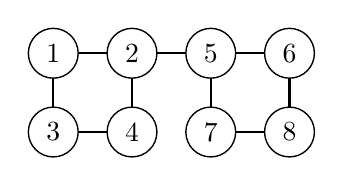
\begin{tikzpicture}
      \Vertex[x=0,y=0]{1}
      \Vertex[x=1,y=0]{2}
      \Vertex[x=0,y=-1]{3}
      \Vertex[x=1,y=-1]{4}
      \Vertex[x=2,y=0]{5}
      \Vertex[x=3,y=0]{6}
      \Vertex[x=2,y=-1]{7}
      \Vertex[x=3,y=-1]{8}
      \Edges(1, 2, 4, 3, 1)
      \Edges(2, 5, 6, 8, 7, 5)
    \end{tikzpicture}
  \end{center}
\end{eg}

An \emph{isopertimetric inequality}\index{isoperimetric inequality} of \(G\) is an inequality of the form
\[
  b(A) \geq f(|A|)
\]
for \(A \subseteq V(G)\). This should be a ``good'' (at least nontrivial) inequality, which warrants that such an inequality should decribe a fixed graph, and not applicable to graphs in general.

To minimise the size \(b(A)\) is equivalently to (and usually easier to) the size of

\begin{definition}[neighbourhood]
  A \emph{neighbourhood} of \(A\)
  \[
    N(A) = A \cup b(A) = \{x \in G: d(x, A) \leq 1\}
  \]
  where \(d\) the usual graph distance.
\end{definition}

A natural guess for boundary minimising \(A\) is often
\[
  B(x, r) = \{y \in G: d(x, y) \leq r\}.
\]
Let's test it. Take \(|A| = 4\) in \(Q_3\). Then in the discrete \(A\) is either a hyperplane or a ball. We have \(|b(A)| = 3\) for ball and \(|b(A)| = 4\) for hyperplane. This works so we conjecture that ``balls are the best'', i.e.\ if \(|A| = |X^{(\leq r)}|\) then \(|N(A)| \geq |X^{(\leq r + 1)}|\). When \(|A|\) is strictly between \(\sum_{i = 0}^r \binom{n}{i}\) and \(\sum_{i = 0}^{r + 1} \binom{r}{i}\), conjecture that \(b(A)\) is minimised if \(A = X^{(\leq r)} \cup B\) for some \(B \subseteq X^{(r + 1)}\). This is a \emph{Hamming ball}\index{Hamming ball}. Note that if we assume this result then
\[
  N(A) = X^{(\leq r + 1)} \cup \shadow^+ B,
\]
so by Krustal-Katona, we'd take \(B\) to be an initial segment of lex on \(X^{(r + 1)}\). This strongly suggests that there is a ordering on \(\powerset(X)\), where subsets are ordered by sizes and lex is used to decide order amongs subsets of equal size, such that the boundary minimising sets are the initial segments of this order.

\begin{definition}[simplicial order]\index{simplicial order}
  The \emph{simplicial order} on \(Q_n\) is defined by \(x < y\) if either \(|x| \leq |y|\) or \(|x| = |y|\) and \(x < y\) in lex.
\end{definition}

\begin{notation}
  In this chapter we use roman instead of curly upper case letters such as \(A, B\) to denote a family of subsets of \(X\), and lower case letters such as \(x, y\) to denote element of \(X\). This is compatible with the vertex convention in graph theory.
\end{notation}

Our aim is to show that initial segments of simplicial are the best. As we have Krustal Katona at disposal, we would like to do similar ``compressions'' to move a set ``closer'' to Hamming ball. In the proof of Krustal Katona the compressions \(C_{UV}\) can be seen as operations of dimension \(|U|\) in the discrete cube. Here we consider ``codimension \(1\)'' compression.

\begin{definition}[section]\index{section}
  Given \(A \subseteq Q_n\) and \(1 \leq i \leq n\), the \emph{\(i\)-sections} are the set systems \(A^{(i)}_+, A^{(i)}_- \subseteq \powerset(X - i)\), thought as \(Q_{n - 1}\), given by
  \begin{align*}
    A^{(i)}_+ &= \{x \in A: i \notin x\} \\
    A^{(i)}_- &= \{x - \{i\}: x \in A, i \in x\}
  \end{align*}
  If it is clear which \(i\) is being considered we may omit the superscripts for simplicity.
\end{definition}

\begin{definition}[\(i\)-compression]\index{\(i\)-compression}
  Define the \emph{\(i\)-compression} \(C_i(A)\) of \(A\) by compression on its \(i\)-sections, i.e.\ \(C_i(A)^{(i)}_+\) is initial segment of \(Q_{n - 1}\) of size \(|A^{(i)}_+|\) and \(C_i(A)^{(i)}_-\) is initial segment of \(Q_{n - 1}\) of size \(|A^{(i)}_-|\).
\end{definition}

\begin{eg}
  (graph)
\end{eg}

Certainly \(|C_i(A)| = |A|\). Moreover, \(C_i(A)\) ``looks more like'' the initial segment of simplicial than \(A\) did.

Say \(A\) is \emph{\(i\)-compresses} if \(C_i(A) = A\).

\begin{theorem}[Harper]\index{Harper's theorem}
  Let \(A \subseteq Q_n\) and \(C\) be the inital segment of simplicial order with \(|C| = |A|\). Then
  \[
    |N(A)| \geq |N(C)|.
  \]
\end{theorem}

Same as in Krustal Katona, what we are really interested in is the ``nice'' size, i.e.\ if \(|A| \geq \sum_{i = 0}^r \binom{n}{i}\) then
\[
  |N(A)| \geq \sum_{i = 0}^{r + 1} \binom{n}{i}.
\]

\begin{remark}\leavevmode
  If \(A\) is a Hamming ball then done by Krustal Katona. Conversely, Harper implies Krustal-Katona. Indeed, given \(B \subseteq X^{(r)}\), apply Harper to \(A = B \cup X^{(\leq r - 1)}\).
\end{remark}

% Note to self: proofread until told to stop

\begin{proof}
  Induction on \(n\): \(n = 1\) is trivial. Given \(A \subseteq Q_n\) where \(n > 1\), fix \(1 \leq i \leq n\). Claim that
  \[
    |N(C_i(A))| \leq |N(A)|.
  \]
  \begin{proof}
    % TODO: proofread this proof
    Write \(B = C_i(A)\). Given an element in the neighbourhood of \(A\), it is either in the downstairs part \(A_-\) or the upstairs part \(A_+\) so
    \[
      |N(A)| = |A_+ \cup N(A_-)| + |A_- \cup N(A_+)|
    \]
    Similarly
    \[
      |N(B)| = |B_+ \cup N(B_-)| + |B_- \cup N(B_+)|.
    \]
    Now \(|B_+| = |A_+|\) and \(|N(B_-)| \leq |N(A_-)|\) by induction. But \(N(B_-)\)  is an initial segment of simplicial (on \(Q_{n - 1}\)), as is \(B_+\), so \(N(B_-)\) and \(B_+\) are nested. Hence
    \[
      |B_+ \cup N(B_-)| \leq |A_+ \cup N(A_-)|
    \]
    and similarly
    \[
      |B_- \cup N(B_+)| \leq |A_- \cup N(A_+)|
    \]
    thus
    \[
      |N(B)| \leq |N(A)|.
    \]
  \end{proof}

  Among all \(B \subseteq Q_n\) with \(|B| = |A|\) and \(|N(B)| \leq |N(A)|\), choose one with \(\sum_{x \in B} f(x)\) minimal, where \(f(x)\) is position of \(x\) in simplicial ordering of \(Q_n\). Then \(B\) is \(i\)-compressed for all \(i\).

  Must such \(B\) be an initial segment of simplicial? Unfortunately, no. For example \(A = \{\emptyset, 1, 2, 12\} \subseteq Q_3\). However, we have

  \begin{lemma}
    Let \(B \subseteq Q_n\) be \(i\)-compressed for all \(i\) but not an initial segment of simplicial order. Then if \(n\) is odd, say \(n = 2k + 1\), we have
    \[
      B = X^{(\leq k)} - \underbrace{\text{ last \(k\)-set }}_{(k + 2)(k + 3) \dots (2k)(2k + 1)} \cup \underbrace{\text{ first \((k + 1)\)-set}}_{12\dots k(k + 1)}
    \]
    whereas if \(n\) is even, say \(n = 2k\), we have
    \[
      B = X^{(\leq k - 1)} \cup \{x \in X^{(k)}: 1 \in x\} - \underbrace{\text{ last \(k\)-set with \(1\) }}_{1(k + 2)(k + 3) \dots (2k)} \cup \underbrace{\text{ first \(k\)-set without \(1\)}}_{234\dots k (k + 1)}
    \] 
  \end{lemma}
  Then done as in each case have \(|N(B)| \geq |N(C)|\).

  \begin{proof}
    Have \(x \notin B, y \in B\) for some \(x < y\) in simplicial. Cannot have \(i \in X, i \in y\) as \(B\) is \(i\)-compressed, and cannot have \(i \notin x, i \notin y\), again as \(B\) is \(i\)compressed. So for each \(i\), \(i\) belongs to exactly one of \(x\) or \(y\). Thus \(y = x^c\).

    Hence for each \(y \in B\), at most one of \(x < y\) has \(x \notin B\) (namely \(y^c\)) and for each \(x \notin B\), at most one of \(y > x\) has \(y \in B\) (namely \(x^c\)). Hence
    \[
      B = \{z: z \leq y\} - \{x\}
    \]
    where \(x\) is the immediate predecessor of \(y\) and \(x = y^c\).

    But then \(x\) is the last \(k\)-set (if \(n = 2k + 1\)) or last \(k\)-set containing \(1\) (if \(n = 2k\)), by definition of simplicial ordering.
  \end{proof}
\end{proof}

\begin{remark}\leavevmode
  \begin{enumerate}
  \item It is also possible to prove Harper by \(UV\)-compression.
  \item We can also use these ``codimension \(1\)'' compressions to prove Krustal Katona directly.
  \end{enumerate}
\end{remark}

In analysis, we often use isoperimetric inequality in blow-up form, e.g.\ give a disk, if we expand it a little bit by \(\varepsilon > 0\) at some point then the resulting shape has perimeter at least as large as that of the disk.

\begin{definition}[\(t\)-neighbourhood]
  For \(A \subseteq Q_n\), the \emph{\(t\)-neighbourhood} of \(A\) is
  \[
    A_{(t)} = N^t(A) = \{x \in Q_n: d(x, A) \leq t\}
  \]
\end{definition}

\begin{corollary}
  Let \(A \subseteq Q_n\) with \(|A| = |X^{(\leq r)}|\). Then for \(1 \leq t \leq n - r\), have
  \[
    |A_{(t)}| \geq |X^{(\leq r + t)}|.
  \]
\end{corollary}

\begin{proof}
  Harper and induction.
\end{proof}

To get a better for for what the corollary is saying, we'll need some estimates and things like \(\sum_{i = 0}^r \binom{n}{i}\).
% c.f. central limit theorem

\begin{proposition}
  Let \(0 < \varepsilon < \frac{1}{4}\), then
  \[
    \sum_{i = 0}^{\floor{(\frac{1}{2} - \varepsilon) n}} \binom{n}{i} < \frac{1}{\varepsilon} \exp (- \frac{\varepsilon^2 n}{2}) 2^n.
  \]
\end{proposition}

i.e.\ for fixed \(\varepsilon\), the sum is an exponentially small fraction of \(2^n\)

In standard deviation language, going \(\sim \varepsilon\) standard deviates from mean

\begin{proof}
  For \(i \leq (\frac{1}{2} - \varepsilon) n\),
  \[
    \frac{\binom{n}{i - 1}}{\binom{n}{i}}
    = \frac{i}{n - i + 1}
    \leq \frac{\frac{1}{2} - \varepsilon}{\frac{1}{2} + \varepsilon}
    = 1 - \frac{2\varepsilon}{\frac{1}{2} + \varepsilon}
    \leq 1 - 2\varepsilon.
  \]
  Hence by comparison with geometric progression
  \[
    \sum_{i = 0}^{\floor{(\frac{1}{2} - \varepsilon) n}} \binom{n}{i}
    \leq \frac{1}{2\varepsilon} \binom{n}{\floor{(\frac{1}{2} - \varepsilon) n}}.
  \]
  Similarly
  \[
    \binom{n}{\floor{(\frac{1}{2} - \varepsilon)n}}
    \leq (1 - \varepsilon)^{\varepsilon n / 2 - 1} \binom{n}{\floor{(\frac{1}{2} - \frac{\varepsilon}{2}) n}} %\text{ by replacing \varepsilon with \varepsilon/2}
    \leq 2(1 - \varepsilon)^{\varepsilon n/2} 2^n
    \leq 2 \exp{-\varepsilon \varepsilon n /2} \cdot 2^n
  \]
  Therefore
  \[
    \sum_{i = 0}^{\floor{(\frac{1}{2} - \varepsilon)n}} \leq \frac{1}{2\varepsilon} 2 \exp{- \varepsilon^2n /2} 2^n.
  \]
\end{proof}

% end of proofread

Missed a lecture on 06/11/18










\printindex
\end{document}

% Three parts:
% Chapter 1: set systems
% Chapter 2: isoperimetric inequalities
% Chapter 3: projections
% Books: Combinatorics, Bollobas, CUP 1986, excellent for Chapter 1 and Chapter 2 (and gentle!) and for future development of the course;
% Combinatorics of finite sets, Anderson, OUP 1987, simple and clear, good for Chapter 1